\documentclass[12pt,a4paper]{ctexart}

\usepackage[margin=2.2cm]{geometry}
\usepackage{amsmath,amssymb}
\usepackage{graphicx}
\usepackage{booktabs}
\usepackage{multirow}
\usepackage{enumitem}
\usepackage{float}
\usepackage{hyperref}

\graphicspath{{../figures/}}

\title{\bfseries 微网与外部电网电力调控策略}
\author{}
\date{}

\begin{document}

\maketitle

\begin{center}
\textbf{摘\quad 要}
\end{center}

\noindent
微网为消纳光伏、减少并网问题而快速发展的小区发电用电系统。本文建立"满足负荷、最小化购电
费用"的微网购电/储能充放优化模型，并按信息复杂度递进四个子问题：
(1)~确定性日前计划；(2)~固定电价下日前计划+紧急购电（5倍价）；(3)~基于
0:00、6:00、12:00、18:00 四次光伏预报的滚动调整购电；(4)~波动电价下重算第(2)、(3)问。
各问均化为以十分钟为时段、以储能荷电状态（SOC）递推的线性规划（LP）；
充放互斥天然成立、弃光与购电非负。储能容量 12000\,kWh、运行区间 1200--10800\,kWh、
充放电效率 0.9、日初与日末储电量均取 6000\,kWh。

在附件数据上求解得到：
\textbf{问题一}（附件1单日）全天计划购电 \textbf{86108\,kWh}、购电费 \textbf{55363\,元}，
0:00 与 24:00 储电均为 6000\,kWh；
\textbf{问题二}（全年）计划购电 24945\,MWh，紧急购电 \textbf{30102\,kWh}（紧急费 150833\,元），
总费用 \textbf{15.892 百万元}；
\textbf{问题三}（四次预报滚动调整）紧急购电骤降至 \textbf{808\,kWh}（紧急费 3785\,元），
但调整偏差结算约 90.5 万元，总费用升至 \textbf{16.650 百万元}；
\textbf{问题四}（动态电价）result4-2 总费 16.283 百万、result4-3 总费 16.969 百万元。

\noindent 关于"是否引入其他时刻预报"：从降低紧急购电（约 -97\%）、提高供电可靠性的角度看有必要引入；
若仅以总购电费用最小为目标，多次调整的 $1.5\times$ 上调结算成本可能抵消其收益，本文给出量化依据。

\begin{figure}[H]\centering
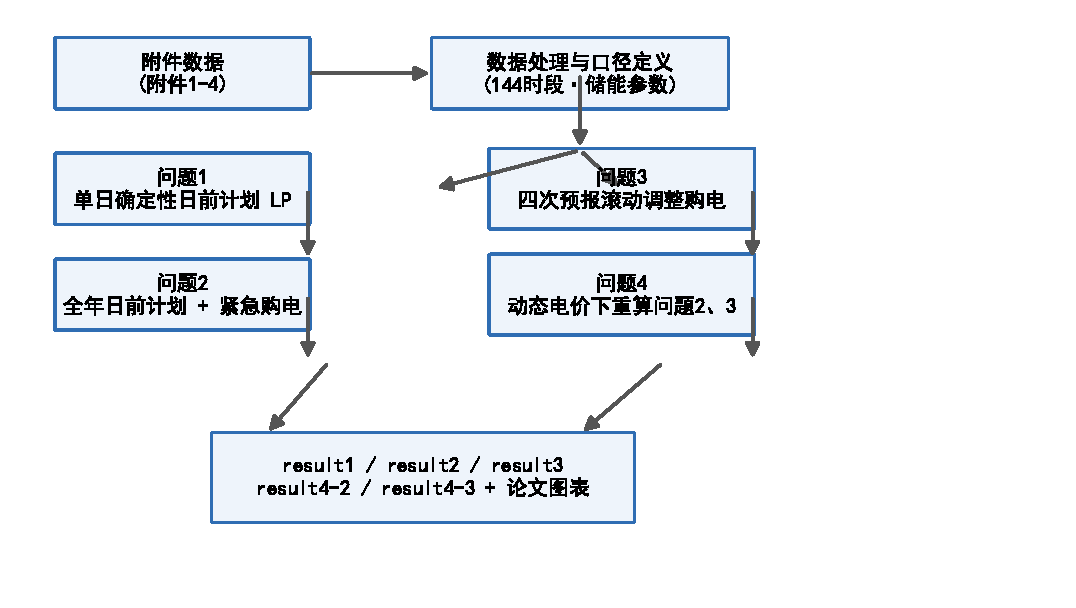
\includegraphics[width=0.85\textwidth]{fig_roadmap.pdf}
\caption{解题技术路线图}\label{fig:roadmap}
\end{figure}

\section{问题重述与背景}
微网与外网调控目的是利用小区负载、光伏发电量和储能当前储电量，尽可能精准地给出微网购电量
与储能充放电量，使微网供电既满足小区负载，又尽可能节省购电费用。
\nobreak
\begin{figure}[H]\centering
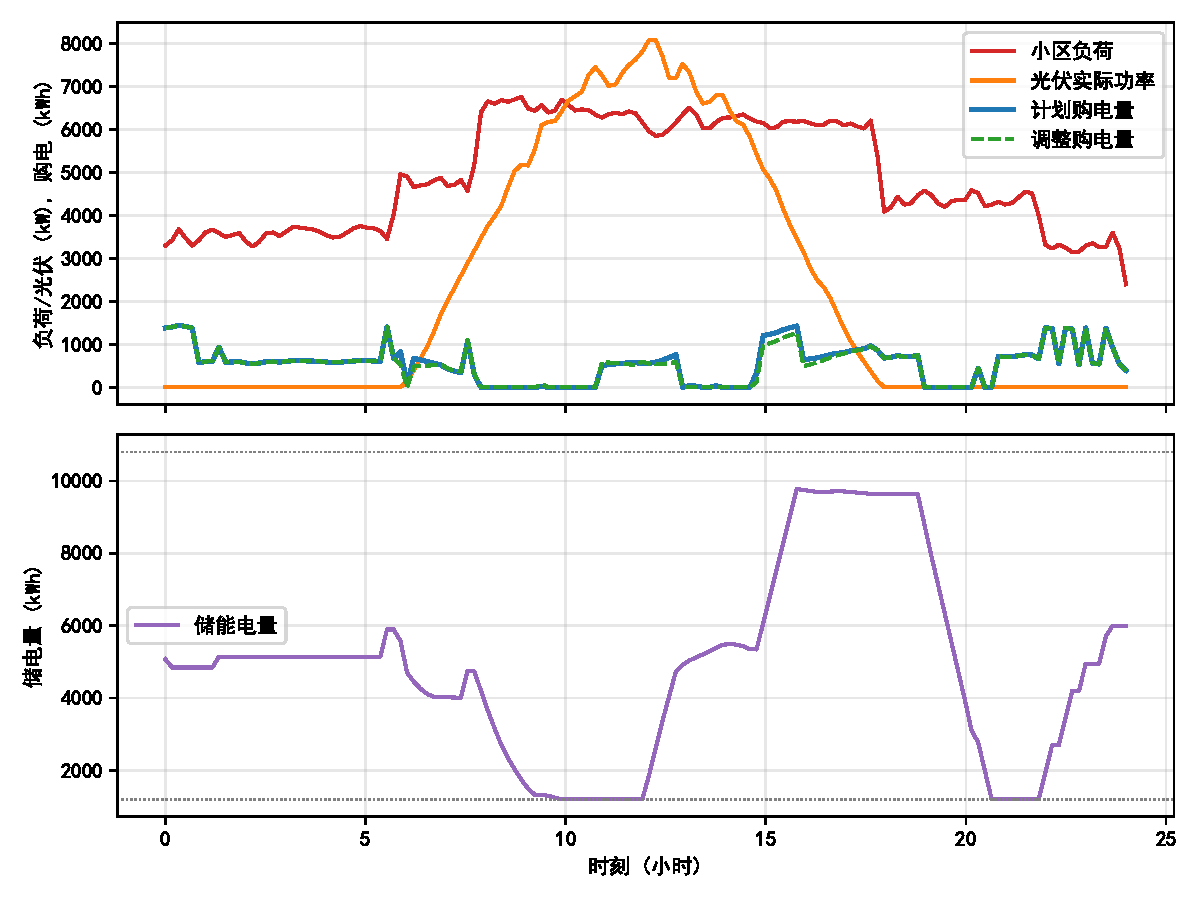
\includegraphics[width=0.85\textwidth]{fig_repday.pdf}
\caption{代表日(2025-03-20)的负荷、光伏实际、计划购电与调整购电、储能电量}\label{fig:repday}
\end{figure}

\section{模型假设与符号}
\begin{itemize}[itemsep=1pt]
  \item 储能容量 12000\,kWh，运行区间 1200--10800\,kWh，充放电效率 0.9，
        最大充放电功率 5000\,kW（十分钟时段最大能量 833.33\,kWh）；日初与日末储电量相等并取 6000\,kWh。
  \item 微网供电不低于（取等于）小区负荷，购电量非负（不外售），光伏过剩可弃光。
  \item 附件3 整点预报线性插值到十分钟网格；问题3按时序固定已执行时段，仅优化剩余时段。
\end{itemize}
符号：$q_t$ 计划购电量(kWh)；$C_t,D_t$ 充/放电量(kWh)；$E_t$ 储电量(kWh)；
$G_t,L_t,p_t$ 光伏/负荷(kW)、电价；$e_t^{em}$ 紧急购电量；$s_t^-,s_t^+$ 调整偏差负/正分量。

\section{问题一：确定性日前的计划购电}
目标与约束（$t=1,\dots,144$，$\Delta t=1/6$ h）：
\begin{align}
  &\min J_1 = \sum_{t=1}^{144} p_t\,q_t \label{eq:P1obj}\\
  &E_t = E_{t-1}+0.9\,C_t - D_t/0.9,\quad 1200\le E_t\le 10800 \label{eq:soc}\\
  &q_t + G_t\,\Delta t + D_t = L_t\,\Delta t + C_t + \mathrm{curt}_t,\quad q_t,\mathrm{curt}_t\ge 0 \label{eq:bal}\\
  &0\le C_t,D_t\le 833.33,\quad E_0=E_{144}=6000. \label{eq:cap}
\end{align}
同一时段充/放各承担 $\pm p_t$ 且无售电收益、每次启停损耗 $0.9\eta$，故最优解天然充放互斥，
问题一是纯 LP。求解得：全天计划购电 \textbf{86108\,kWh}、购电费 \textbf{55363\,元}；
储能充电 17837、放电 14448\,kWh；0:00 与 24:00 储电均 6000\,kWh。结果填入 result1。

\begin{figure}[H]\centering
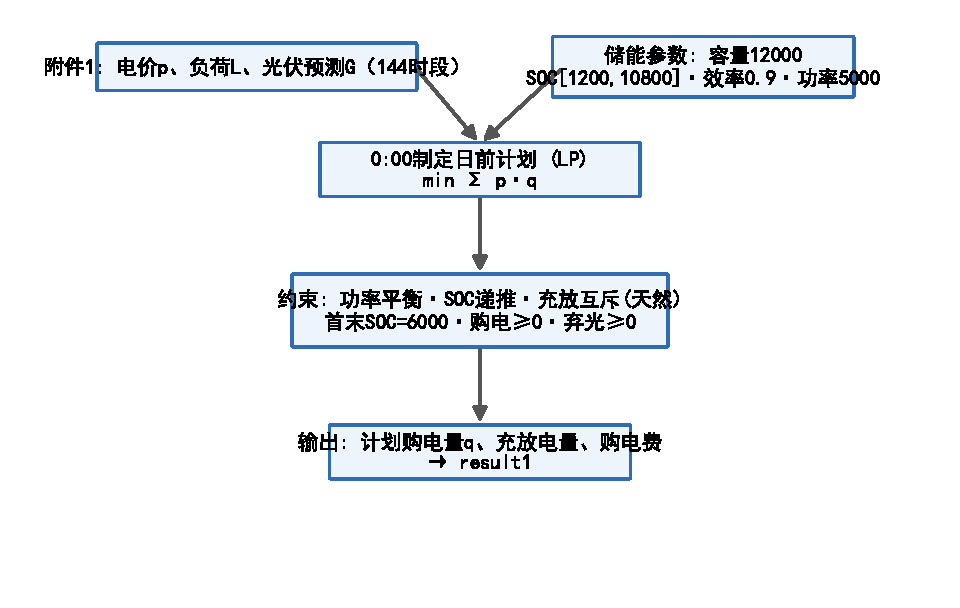
\includegraphics[width=0.7\textwidth]{fig_flow_q1.pdf}
\caption{问题一计划购电求解流程}\label{fig:q1}
\end{figure}

\section{问题二：固定电价下日前计划与紧急购电}
0:00 依附件3预报定计划 $q_t^{DA}$；实际执行用附件2实际光伏与储能再调度，供电不足时以
$5p_t$ 紧急购电：
\begin{equation}
\min J_2 = \sum_t p_t\,q_t^{DA} + 5\sum_t p_t\,e_t^{em}
\end{equation}
约束同问题一，且含 $G_t^{act}$ 与 $e_t^{em}\ge0$。全年：计划购电 24945\,MWh，
紧急购电 30102\,kWh（紧急费 150833\,元），总费 15.892 百万元。结果填入 result2。

\section{问题三：四次预报的滚动调整购电}
0:00 定计划 $q^{DA}$；6:00/12:00/18:00 以最新预报优化剩余时段得调整购电量 $a_t$；
$a_t$ 高于计划的部分按 $1.5p_t$、低于计划的部分按 $0.5p_t$ 结算，实际缺口按 $5p_t$ 紧急购电：
\begin{align}
&\min J_3 = \sum_t p_t\,q_t^{DA}+\sum_t p_t(0.5\,s_t^-+1.5\,s_t^+)+5\sum_t p_t\,e_t^{em}\\
&a_t - q_t^{DA} = s_t^+ - s_t^-,\quad s_t^\pm\ge0
\end{align}
三次滚动调整后紧急购电由 30102 降至 808\,kWh（紧急费 150833$\to$3785 元），
但偏差结算约 90.5 万元，总费升至 16.650 百万元。结果填入 result3。

\begin{figure}[H]\centering
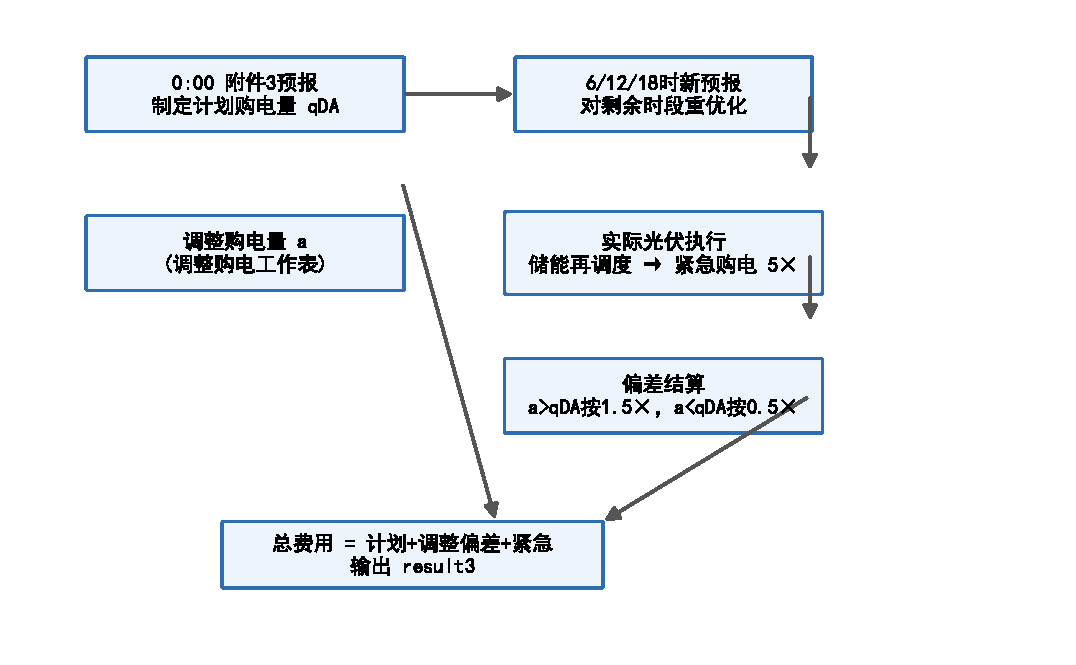
\includegraphics[width=0.8\textwidth]{fig_flow_q3.pdf}
\caption{问题三滚动购电与偏差结算流程}\label{fig:q3}
\end{figure}
\begin{figure}[H]\centering
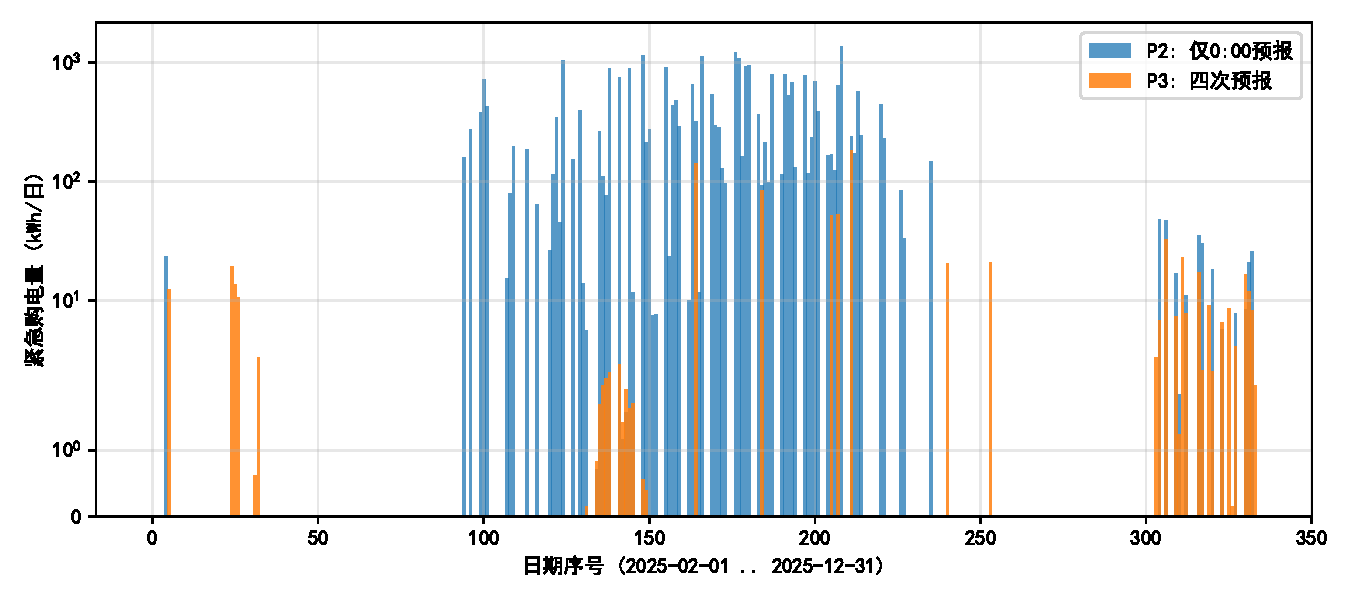
\includegraphics[width=0.86\textwidth]{fig_emergency.pdf}
\caption{全年逐日紧急购电量：问题2（仅0:00预报）与问题3（四次预报）对比}\label{fig:em}
\end{figure}

\section{问题四：波动电价下重算问题二、问题三}
以附件4动态电价 $p_t^{dyn}$ 替换固定电价，结构同问题二/三：
\begin{equation}
J_{4}=\sum_t p_t^{dyn}q_t^{DA}+5\sum_t p_t^{dyn}e_t^{em}
\qquad(\text{问题2口径，问题3再加 }\sum_t p_t^{dyn}(0.5s_t^-+1.5s_t^+)).
\end{equation}
全年：result4-2 总费 16.283 百万元、result4-3 总费 16.969 百万元。
动态价下峰谷差拉大，储能"低价充电、高价放电"的移峰收益更明显（如图 \ref{fig:price}）。

\begin{figure}[H]\centering
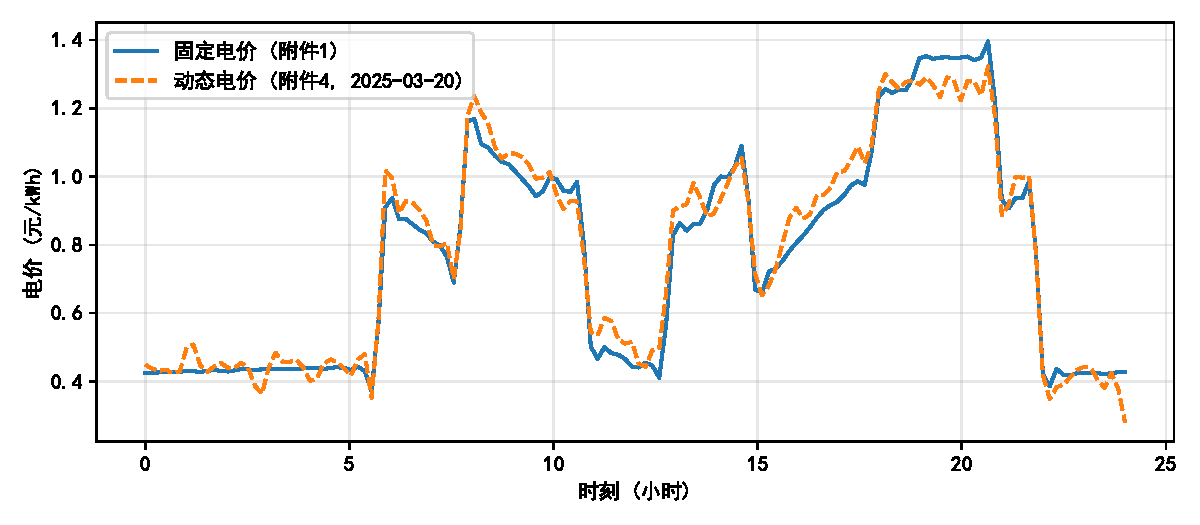
\includegraphics[width=0.78\textwidth]{fig_price.pdf}
\caption{固定电价（附件1）与动态电价（附件4，2025-03-20）对比}\label{fig:price}
\end{figure}

\section{灵敏度分析与模型评价}
\begin{itemize}[itemsep=1pt]
  \item 储能效率 0.85/0.90/0.95：效率越高储运越经济，购电费单调略降。
  \item 高光伏日必须允许弃光，否则模型不可行；SOC 区间越宽可用储能越大、购电费越低。
  \item 动态 vs 固定电价：峰谷差放大，储能移峰节费更显著。
  \item 优点：均为 LP，可复现、可逐日并行、求解快。
  \item 不足：未计储能寿命损耗与弃光损失；调整为启发式滚动调度口径。
  \item 推广：引入鲁棒/随机优化刻画预测误差，纳入储能循环寿命成本。
\end{itemize}

\noindent\textbf{结论}：四问均以十分钟线性规划求得最优购电/充放策略并按要求输出结果文件；
三次预报显著降低紧急购电、提高供电可靠性，但若以总费用最小为首要目标，需权衡调整偏差结算成本。

\end{document}
